\section{Progress}
\label{sec:progress}
\subsection{Weeks 1-2}
During the first 2 weeks of term time was spent on the Specificationa as well as attempting to establish a strong
base to the project in which I can build on for the rest of the project.

\begin{figure}[htbp]
    \centering
    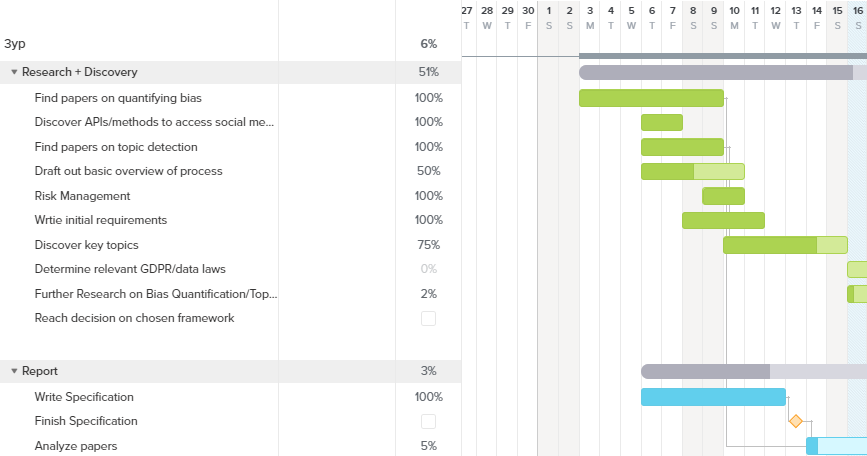
\includegraphics[width=0.5\textwidth]{../images/timetableweek1-2.png}
    \caption{Timetable for weeks 1-2}
    \label{fig:timetableweek1-2}
\end{figure}

As seen from this figure I met most of the deadlines set for the first 2 weeks of the project. I did miss some deadlines
Including: Drafting an overview of the process; Discovering key topics; and starting looking into GDPR and Data Protection laws.
Although it would have been beneficial to have achieved the latter 2 in the list above, the first objective was probably infeasible
for the first 2 weeks of the project - as further research is required to determine where I want this project taking.\\\\

I also completed a few extra tasks slightly early this week. I established an API connection to Twitter as well as reading up on
API access to Facebook and Instagram. As mentioned in my specification, I am going to stick with using Twitter as a base for
this project but may look into using Facebook and Instagram as well.\\\\

Finally I started looking more into the papers I laid out in the spec. Specifically looking into Pythia and how they overcome
the challenge of twitter posts usually being short and not containing much information.

\subsection{Weeks 3-4}
During weeks 3 and 4, time was spent time was spent further working on establishing the goals of the project. It was
decided that the project would be split into 2 parts. The first part would be to create a system that can be used to
analyse twitter posts and determine the topic of the post. I chose to go with a similar method used in Pythia \cite{Pythia}.
The latter stages of the project would involve using the system and analyse how different social media "strategies" affect
the topical bias of a users feed.\\\\

Below is the timetable for weeks 3-4.

\begin{figure}[htbp]
    \centering
    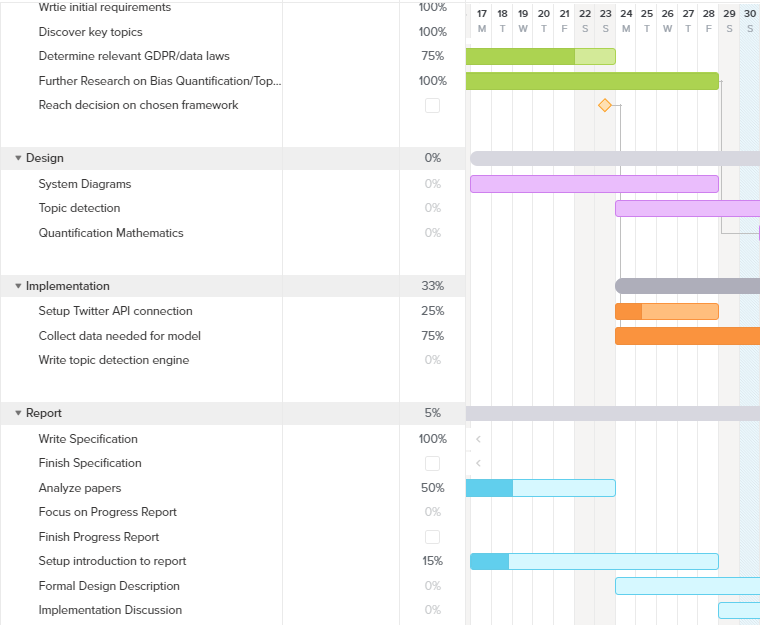
\includegraphics[width=0.5\textwidth]{../images/timetableweek3-4.png}
    \caption{Timetable for weeks 3-4}
    \label{fig:timetableweek3-4}
\end{figure}

As seen from the timetable above, I did not meet all of the deadlines set for weeks 3-4; due to needing to complete more
research on other methods of topic detection (such as Formal Concept Analysis, Clustering, and Latent Dirichlet Allocation),
I spent the week deciding which of these methods would be preferred (As mentioned above).

On top of this, I also gathered the Wikipedia data required for the training of the system. This involved:
\begin{itemize}
    \item Connecting to the Wikipedia API
    \item Searching for the decided upon categories
    \item Selecting 100 pages for each category
    \item Performing some preprocessing on the data
    \begin{enumerate}
        \item removing punctuation
        \item removing numbers
        \item removing excessive whitespace (leaving only spaces)
        \item removing Stopwords
    \end{enumerate}
\end{itemize}
def: Stopwords are words that are commonly used in the English language, but are uninformative \cite{sarica2021stopwords}.\\\\

This process gave us a total of $24,000$ sentences at around $1,000$ per category.


\subsection{Weeks 5-6}
During weeks 5 and 6, time was focussed around BERT. BERT, which stands for Bidirectional Encoder Representations from Transformers,
is a modern model which focusses on the task of language modelling. It is a pre-trained model which can be used to perform more precise
tasks after being fine-tuned \cite{devlin_bert_2019}. Fine-tuning of the model is done by adding a classification layer on top of the
model and training the model on a specific task.\\

The model was fine-tuned on the Wikipedia data gathered in the previous weeks. The model was trained on 24 categories, including:
Politics, Sports, Food, etc. The model was trained for 6 epochs, with a batch size of 32. The single output layer used the
softmax activation function. The model was trained using the Adam optimizer with the sparse categorical cross entropy loss function.\\

The data was split into 80\% training data and 20\% testing data. The model was trained on the training data and then tested on the
test data. Initially, the model was not very impressive, only achieving around 40\% accuracy.
% Insert figure, move onto next page if needed

\begin{figure}[htbp]
    \centering
    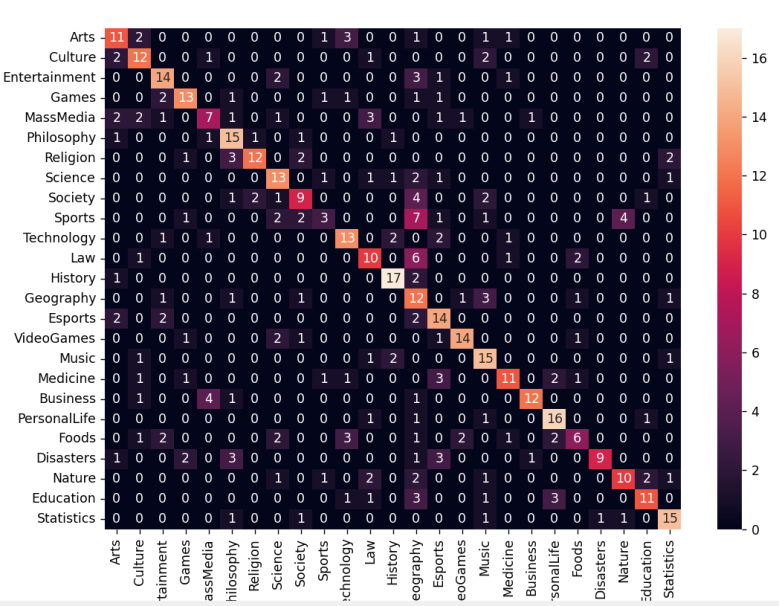
\includegraphics[width=0.5\textwidth]{../images/wiki-confusion.png}
    \caption{Confusion matrix on the Wikipedia data}
    \label{fig:wikiconf}
\end{figure}
Further analysis of the data showed that
the data was of a poor quality; even after the processing, the data still contained meaningless sentences. Take for example:
"51 (1): 209-220.", there is no way of identifying the topic of this sentence. On top of this, the data seemed to be too formal to
be used for analysing social media. Because of these facts, the decision was made to not use Wikipedia data for the training and instead
use Reddit data.\\
Reddit data was chosen as it is a more informal platform and is more likely to contain sentences that are formatted similarly to
other social media sites.\\
The same process as laid out in the previous weeks was followed. The data was gathered, preprocessed. The model was trained and tested
and with the reddit data, had a much higher testing accuracy of around 60\%.
\newpage
\begin{figure}[htbp]
    \centering
    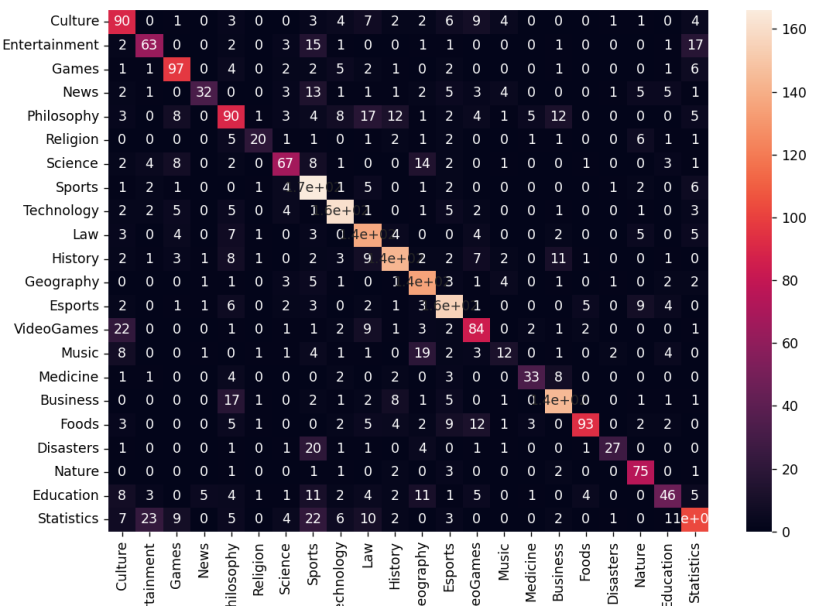
\includegraphics[width=0.5\textwidth]{../images/reddit-confusion.png}
    \caption{Confusion matrix on reddit data}
    \label{fig:reditconf}
\end{figure}

\subsection{Weeks 7-8}
